\documentclass[11pt,a4paper]{article}
\usepackage[margin=1in]{geometry}
\usepackage{amsmath,amssymb,amsthm}
\usepackage{hyperref}
\usepackage{enumitem}
\usepackage{algorithm}
\usepackage{algpseudocode}
\usepackage{tikz}
\usepackage{booktabs}
\usetikzlibrary{arrows.meta,positioning,calc}

\theoremstyle{definition}
\newtheorem{definition}{Definition}
\newtheorem{construction}{Construction}
\newtheorem{property}{Property}

\hypersetup{colorlinks=true, linkcolor=blue!60!black, citecolor=blue!60!black, urlcolor=blue!60!black}

\title{Shielded Payments for Decentralized Cloud Services:\\Anonymous Pay-Per-Use via Cross-Chain\\Shielded Pools, Prepaid Credits, and Rate-Limiting Nullifiers}

\author{
  Drew Stone\\
  \texttt{drew@tangle.tools}\\
  Tangle Network
}

\date{March 2026}

\begin{document}
\maketitle

\begin{abstract}
We present a privacy-preserving payment system for decentralized cloud services---LLM inference, image generation, compute---where users pay anonymously and operators serve requests without learning the payer's identity. The system composes three layers: (1)~a cross-chain UTXO-based shielded pool~\cite{webb} with variable-amount JoinSplit transactions and multi-stablecoin wrapping, (2)~a stateless gateway contract that bridges anonymous partial withdrawals to Tangle's Blueprint service lifecycle, and (3)~a prepaid credit scheme where a single zero-knowledge proof funds an account from which many jobs are authorized via EIP-712 signatures. We describe the deployed system (v1) and a planned upgrade to per-request unlinkability via Rate-Limiting Nullifiers~\cite{rln} composed with the existing audited VAnchor circuit (v2). The v1 construction requires no modifications to Tangle's audited core contracts and introduces under 1,000 lines of new Solidity.
\end{abstract}

\tableofcontents

\section{Introduction}

Every major AI inference provider---OpenAI, Anthropic, Google---requires account creation, identity verification, and traceable payment. A developer querying an LLM for code review, legal analysis, or medical information creates a permanent record linking their identity to every prompt. Decentralized alternatives inherit the same problem: on-chain payments link wallet addresses to service consumption with full public auditability.

This is not hypothetical. Inference providers can profile users by query content, timing, and volume. Employers can monitor which employees use AI assistance. Competitors can observe which organizations are training custom models. The payment trail is the surveillance vector.

Buterin and Crapis~\cite{zkapi} proposed \emph{ZK API Usage Credits}: deposit into a smart contract, generate a zero-knowledge proof per API call to authorize payment without revealing identity. The proposal achieves strong privacy---per-request unlinkability via Rate-Limiting Nullifiers---but requires a Groth16 proof per API call ($\sim$640ms generation, $\sim$300k gas on-chain).

We present a two-phase approach that ships immediately (v1) while providing a clear upgrade path to per-request unlinkability (v2):

\begin{description}[nosep, leftmargin=1.5cm]
  \item[v1 (deployed):] One ZK proof funds a pseudonymous credit account. Many ECDSA signatures authorize individual job payments ($\sim$50k gas each). Requests within a credit session share a pseudonym; sessions are unlinkable.
  \item[v2 (planned):] Each request carries its own RLN-based ZK proof, verified off-chain by the operator. Zero on-chain transactions per request. Full per-request unlinkability. The RLN circuit~\cite{rln} composes with the audited VAnchor circuit~\cite{webb,veridise} with $\sim$100 new constraints.
\end{description}

\subsection{Contributions}

\begin{enumerate}[nosep]
  \item A UTXO-based privacy model with partial withdrawals producing unlinkable change notes, enabling incremental spending from a single deposit.
  \item A two-phase payment scheme: one ZK proof amortized over many ECDSA-signed payments (v1), upgradeable to per-request RLN proofs verified off-chain (v2).
  \item A gateway architecture bridging VAnchor shielded pools to Tangle's service lifecycle with zero core protocol modifications.
  \item Multi-asset wrapping (USDC, USDT, DAI $\to$ single pool token) maximizing the anonymity set.
  \item A cross-chain bridge via LayerZero V2 with dynamic edge addition, supporting deposits on 8 chains.
  \item An audit-preserving circuit composition strategy where the v2 upgrade reuses audited sub-circuits (VAnchor~\cite{veridise}, RLN~\cite{rlnaudit}) with $\sim$100 lines of new glue constraints.
\end{enumerate}

\section{Preliminaries}

We adopt notation from the Webb Protocol~\cite{webb}. Let $H : \mathbb{F}_p^* \to \mathbb{F}_p$ denote Poseidon~\cite{poseidon}, a zkSNARK-friendly hash over the BN254 scalar field.

\begin{definition}[UTXO Commitment]
A commitment to a UTXO with chain identifier $i$, value $v$, public key $\mathsf{pk} = H(\mathsf{sk})$, and blinding factor $r \xleftarrow{\$} \mathbb{F}_p$ is:
$$\mathsf{cm} = H(i, v, \mathsf{pk}, r)$$
\end{definition}

\begin{definition}[Nullifier]
The nullifier for commitment $\mathsf{cm}$ at Merkle path index $j$, with hash-based signature $\sigma = H(\mathsf{sk}, j, \mathsf{cm})$, is:
$$\mathsf{sn} = H(\mathsf{cm}, j, \sigma)$$
Binding $\sigma$ to the secret key prevents nullifier grinding by parties who observe commitments but do not hold $\mathsf{sk}$.
\end{definition}

\begin{definition}[Cross-Chain Merkle Membership]
Given Merkle roots $\mathbf{MR} = \{\mathsf{MR}_1, \ldots, \mathsf{MR}_k\}$ from $k$ connected anchor instances, commitment $\mathsf{cm}$ satisfies membership if:
$$\mathsf{reconstruct}(\mathsf{cm}, \mathsf{path}(\mathsf{cm}), H) \in \mathbf{MR}$$
The circuit is compiled with a fixed $k$ (currently $k=8$). Unoccupied edge slots are filled with a deterministic zero hash. New chains are added on-chain via \texttt{addEdge} without circuit recompilation or redeployment.
\end{definition}

\section{System Architecture (v1)}

\begin{center}
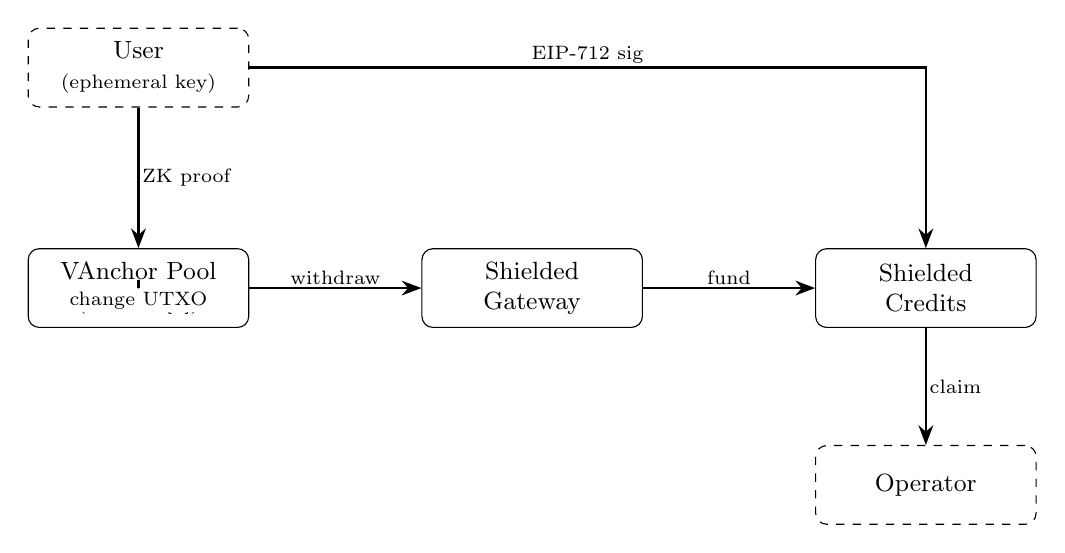
\begin{tikzpicture}[
  box/.style={draw, rounded corners, minimum width=2.8cm, minimum height=1cm, align=center, font=\small},
  arr/.style={-{Stealth[length=2.5mm]}, thick},
  lbl/.style={font=\scriptsize, fill=white, inner sep=1pt}
]
  \node[box] (pool) at (0,0) {VAnchor Pool\\{\scriptsize (audited~\cite{webb})}};
  \node[box] (gw) at (5,0) {Shielded\\Gateway};
  \node[box] (credits) at (10,0) {Shielded\\Credits};
  \node[box, dashed] (user) at (0,2.8) {User\\{\scriptsize (ephemeral key)}};
  \node[box, dashed] (op) at (10,-2.5) {Operator};

  \draw[arr] (user) -- node[lbl, right] {ZK proof} (pool);
  \draw[arr] (pool) -- node[lbl, above, midway] {withdraw} (gw);
  \draw[arr] (gw) -- node[lbl, above, midway] {fund} (credits);
  \draw[arr] (user) -| node[lbl, above, near start] {EIP-712 sig} (credits);
  \draw[arr] (credits) -- node[lbl, right, midway] {claim} (op);

  \draw[arr, dashed] (pool) to[bend right=50] node[lbl, below] {change UTXO} (pool);
\end{tikzpicture}
\end{center}

\subsection{UTXO Model and Partial Withdrawals}

The VAnchor~\cite{webb} implements a UTXO-based shielded pool with JoinSplit transactions (2-in-2-out or 16-in-2-out). Unlike fixed-denomination mixers (e.g., Tornado Cash~\cite{tornado}), each UTXO carries an arbitrary value, enabling partial withdrawals:

\begin{enumerate}[nosep]
  \item User holds $\mathsf{UTXO}(v)$ in the pool (e.g., $v = 100$ USDC).
  \item User generates a Groth16 proof spending $\mathsf{UTXO}(100)$ with outputs:
  \begin{itemize}[nosep]
    \item Withdrawal of 10 to the gateway ($\mathsf{extAmount} = -10$)
    \item Change $\mathsf{UTXO}(90)$ re-shielded in the pool
  \end{itemize}
  \item The circuit enforces conservation: $\mathsf{public\_amount} + \sum v_{\mathsf{in}} = \sum v_{\mathsf{out}}$.
  \item The spent UTXO's nullifier is marked on-chain. The change UTXO has a fresh commitment with fresh blinding---\textbf{unlinkable to the original deposit or prior withdrawals}.
\end{enumerate}

The user repeats this process for each credit session. Each withdrawal consumes a different UTXO, produces a different nullifier, and creates a different change commitment. An observer sees $n$ withdrawals from the pool but cannot determine whether they originate from one depositor or $n$ different depositors.

\subsection{Shielded Gateway}

The \texttt{ShieldedGateway} is a stateless proxy between the VAnchor and Tangle's service layer. It executes a VAnchor withdrawal (validating the Groth16 proof and marking nullifiers on-chain), receives tokens, and atomically forwards them to one of:

\begin{itemize}[nosep]
  \item \texttt{shieldedRequestService}: Create a Tangle service instance with the gateway as owner and ephemeral addresses as permitted callers.
  \item \texttt{shieldedFundService}: Top up an existing service's escrow.
  \item \texttt{shieldedFundCredits}: Fund a prepaid credit account (Section~\ref{sec:credits}).
\end{itemize}

\begin{property}[Atomicity]
The gateway holds no funds beyond a single transaction. Token receipt and forwarding occur in the same call. Failure at any point reverts the entire transaction, including the VAnchor withdrawal.
\end{property}

\begin{property}[Non-Linkability]
The gateway stores no persistent state mapping nullifiers to service or credit identifiers. The on-chain trace reveals only the flow $\texttt{VAnchor} \to \texttt{Gateway} \to \texttt{Credits}$, not which depositor initiated it.
\end{property}

\subsection{Shielded Credits}\label{sec:credits}

The core v1 contribution: a prepaid credit system that amortizes one ZK proof across many service invocations.

\begin{definition}[Credit Account]
Identified by $\mathsf{C} = \mathsf{keccak256}(\mathsf{pk}_s \| \mathsf{salt})$ where $\mathsf{pk}_s$ is an ephemeral ECDSA public key and $\mathsf{salt} \xleftarrow{\$} \{0,1\}^{256}$. Account state: $(\mathsf{pk}_s, \mathsf{token}, \mathsf{balance}, \mathsf{nonce})$.
\end{definition}

\begin{definition}[Spend Authorization]
An EIP-712~\cite{eip712} typed signature over:
$$\mathsf{SpendAuth} = \mathsf{Sign}_{\mathsf{sk}_s}\big(\mathsf{C},\; \mathsf{serviceId},\; \mathsf{jobIndex},\; \mathsf{amount},\; \mathsf{operator},\; \mathsf{nonce},\; \mathsf{expiry}\big)$$
The designated $\mathsf{operator}$ is the only address that can claim payment. Claims after $\mathsf{expiry}$ are rejected; unclaimed funds can be reclaimed by anyone via \textsc{ReclaimExpiredAuth}.
\end{definition}

The credit lifecycle proceeds as: \textsc{FundCredits} (pull tokens, initialize account) $\to$ \textsc{AuthorizeSpend} (verify signature, deduct balance, store pending claim) $\to$ \textsc{ClaimPayment} (transfer to operator, require $\mathsf{msg.sender} = \mathsf{operator}$ and $\mathsf{timestamp} \leq \mathsf{expiry}$).

\section{Privacy Analysis}

\subsection{Operator Knowledge Boundary}

\begin{center}
\begin{tabular}{@{}lcc@{}}
\toprule
\textbf{Information} & \textbf{Operator} & \textbf{Chain observer} \\
\midrule
User's wallet address & \texttimes & \texttimes \\
Deposit amount / total shielded balance & \texttimes & \texttimes \\
Which deposit funded this credit account & \texttimes & \texttimes \\
Credit commitment $\mathsf{C}$ & \checkmark & \checkmark \\
Payment amount per job & \checkmark & \checkmark \\
Request content (prompt, image, query) & \checkmark & \texttimes \\
Linkage between jobs within same $\mathsf{C}$ & \checkmark & \checkmark \\
Linkage between different credit accounts & \texttimes & \texttimes \\
\bottomrule
\end{tabular}
\end{center}

The operator knows \emph{what} was requested and \emph{how much} was paid, but not \emph{who} is paying. This is the ``cash at a store'' model: the merchant sees the transaction but cannot trace it to a bank account.

\subsection{Unlinkability Across Sessions}

When credit account $\mathsf{C}_1$ is depleted, the user generates a new partial withdrawal from their shielded UTXO, creating $\mathsf{C}_2$ with a fresh ephemeral key. The two accounts are cryptographically unlinkable because they use different ephemeral keys, different commitments, different nullifiers, and the connecting change UTXO has fresh blinding. The anonymity set is the total number of depositors in the pool.

\subsection{Limitations of v1}

\textbf{Intra-session linkability.} Multiple spends from the same $\mathsf{C}$ are linkable---the commitment is a pseudonym. Full per-request unlinkability requires a ZK proof per request (addressed in v2, Section~\ref{sec:v2}).

\textbf{Operator sees request content.} Payment privacy does not imply computation privacy. TEE-based execution would address this orthogonally.

\textbf{Anonymity set dependence.} Privacy degrades with few depositors. Multi-asset wrapping and cross-chain deposits are designed to grow the set.

\textbf{No IP-level privacy.} Network-layer anonymity (Tor, Nym) is orthogonal and composable.

\section{Upgrade Path: Per-Request Unlinkability via RLN}\label{sec:v2}

\subsection{Motivation}

The v1 system links requests within a credit session. For sensitive workloads---medical queries, legal analysis, investigative journalism---even pseudonymous linkability may be unacceptable. The v2 upgrade eliminates intra-session linkability entirely.

\subsection{Rate-Limiting Nullifiers}

Rate-Limiting Nullifiers (RLN)~\cite{rln} use Shamir's Secret Sharing to enforce rate limits without identity:

\begin{itemize}[nosep]
  \item Each request in epoch $e$ produces nullifier $\mathsf{rlnNull} = H(\mathsf{sk}, e)$ and reveals one Shamir share: $\mathsf{share} = \mathsf{sk} + a \cdot H(\mathsf{message})$ where $a = H(\mathsf{sk}, e)$.
  \item A single request per epoch reveals one share---insufficient to recover $\mathsf{sk}$.
  \item Two requests in the same epoch reveal two shares on a degree-1 polynomial, enabling recovery of $\mathsf{sk}$ and slashing the user's deposit.
  \item Different epochs produce different nullifiers, providing \textbf{per-request unlinkability}.
\end{itemize}

\subsection{Circuit Composition}

The key architectural insight: the VAnchor circuit (audited by Veridise~\cite{veridise}, $\sim$38k constraints) and the RLN circuit (audited by yAcademy~\cite{rlnaudit}, $\sim$5k constraints) are both Groth16 over BN254 using Poseidon. Composing them preserves the audit guarantees of each sub-circuit. The new audit surface is only the glue logic ($\sim$100 constraints):

\begin{construction}[Composed VAnchor-RLN Circuit]\label{con:composed}
The composed circuit includes three sub-circuits:

\medskip\noindent
\textbf{Sub-circuit A (VAnchor, audited):} Proves UTXO ownership, Merkle membership, nullifier correctness, and amount conservation. Outputs: $\mathsf{cm}$, $\mathsf{amount}$.

\medskip\noindent
\textbf{Glue logic (new, $\sim$100 constraints):}
\begin{align}
  \mathsf{identityCommitment} &:= H(\mathsf{cm}) \\
  (\mathsf{epochIndex} + 1) \times C_{\max} &\leq \mathsf{amount} + R \quad\text{(solvency)}
\end{align}
where $R$ is the accumulated refund balance and $C_{\max}$ is the maximum cost per request.

\medskip\noindent
\textbf{Sub-circuit B (RLN, audited):} Takes $\mathsf{identityCommitment}$ as input. Produces $\mathsf{rlnNull} = H(\mathsf{sk}, \mathsf{epoch})$ and Shamir share. Enforces rate-limiting and enables slashing on double-signal.
\end{construction}

\noindent The sub-circuit constraints are \emph{unchanged}---the glue only connects outputs of A to inputs of B and adds the solvency check. Existing audit findings carry over to the composed circuit. Only the glue logic requires new review.

\subsection{v2 Protocol Flow}

\begin{enumerate}[nosep]
  \item \textbf{Deposit} (on-chain, one-time): User deposits stablecoins into the VAnchor pool.
  \item \textbf{Per-request proof} (client-side, $\sim$640ms): User generates a composed VAnchor-RLN proof. The proof demonstrates: UTXO ownership, solvency, and produces an RLN nullifier + Shamir share.
  \item \textbf{Operator verification} (off-chain, $\sim$5ms): Operator checks the proof against the on-chain Merkle root, verifies the nullifier is fresh, and stores the Shamir share.
  \item \textbf{Service delivery}: Operator serves the request.
  \item \textbf{Refund ticket}: Operator signs a refund ticket $r = (C_{\max} - C_{\mathsf{actual}}, \sigma_{\mathsf{server}})$ for unused capacity. The user accumulates refund tickets locally to unlock further requests without additional deposits.
  \item \textbf{Batch settlement} (on-chain, periodic): Operator submits accumulated nullifiers and claims payment in bulk. No per-request on-chain transaction.
  \item \textbf{Slashing}: If a user double-signals in an epoch, two Shamir shares are revealed. Anyone can recover $\mathsf{sk}$ and slash the user's deposit.
\end{enumerate}

\subsection{v1 $\to$ v2 Comparison}

\begin{center}
\begin{tabular}{@{}lcc@{}}
\toprule
& \textbf{v1 (Credits)} & \textbf{v2 (RLN)} \\
\midrule
Per-request proof & ECDSA signature & Groth16 (off-chain) \\
Per-request on-chain tx & $\sim$50k gas & None (batched) \\
Per-request latency & $<$100ms & $\sim$640ms (client) \\
Intra-session linkability & Yes (same $\mathsf{C}$) & No (per-request nullifier) \\
Rate limiting & Nonce ordering & Shamir slashing \\
Refund for unused capacity & No & Yes (server-signed tickets) \\
New audit surface & 1,000 LOC Solidity & $\sim$100 circuit constraints \\
\bottomrule
\end{tabular}
\end{center}

Both versions coexist---operators can accept either v1 SpendAuth or v2 RLN proofs. Users choose their privacy level per request.

\section{Use Cases}

The system targets workloads where \emph{usage patterns} are as sensitive as the data itself.

\paragraph{LLM Inference.}
Developers querying LLMs for code review, legal analysis, or medical triage create prompt histories that reveal strategic intent. Shielded payments decouple the query from the querier.

\paragraph{Image and Video Generation.}
Creative professionals generating images or video may wish to keep their prompts and creative direction private from the service provider and from on-chain observers.

\paragraph{AI Agent Execution.}
Autonomous agents paying for inference, tool use, and compute should not reveal their controller's identity. The agent's on-chain address is decoupled from the entity that funds it.

\paragraph{Fine-Tuning.}
Organizations submitting proprietary datasets for model fine-tuning can prevent competitors from monitoring training activity via payment trails.

\paragraph{General Cloud Compute.}
Any Blueprint-based service---databases, CI/CD, storage, web hosting---can accept shielded payments. The credit system is service-agnostic.

\section{Cross-Chain Architecture}

The VAnchor supports cross-chain deposits via linked Merkle roots relayed through LayerZero V2. A user deposits USDC on Ethereum; the root is relayed to Base; the user withdraws on Base citing the Ethereum root in the membership proof.

The circuit compiles with $\mathsf{maxEdges} = 7$ (8 chains including self). Unoccupied edge slots are filled with deterministic zero hashes. Chains are added dynamically via \texttt{addEdge}---a single multisig transaction that sets the chain mapping, LayerZero peer, and initial Merkle root atomically.

Initial deployment: Ethereum, Arbitrum, Base, Hyperliquid, BSC. Room for 3 additional chains without circuit recompilation.

\section{Cost Analysis}

\begin{center}
\begin{tabular}{@{}lrrl@{}}
\toprule
\textbf{Approach} & \textbf{Per-request gas} & \textbf{Per-request latency} & \textbf{Privacy} \\
\midrule
ZK proof per call~\cite{zkapi} & $\sim$300k (on-chain) & $\sim$640ms & Full \\
VAnchor withdrawal per call & $\sim$300k (on-chain) & $\sim$640ms & Full \\
\textbf{v1: Shielded Credits} & \textbf{$\sim$50k (on-chain)} & $<$\textbf{100ms} & \textbf{Pseudonymous} \\
\textbf{v2: RLN (off-chain)} & \textbf{0 (batched)} & $\sim$\textbf{640ms} & \textbf{Full} \\
x402~\cite{x402} (no privacy) & $\sim$30k (on-chain) & $<$50ms & None \\
\bottomrule
\end{tabular}
\end{center}

The v1 one-time proof cost is amortized over all jobs in a session. A \$50 credit account at \$0.10/call amortizes over 500 calls. The v2 proof cost is per-request but entirely client-side with zero on-chain gas.

\section{Implementation}

The v1 system is deployed as a standalone Foundry project at \texttt{tangle-network/shielded-payment-gateway}. It compiles against the audited protocol-solidity contracts (git submodule, unmodified) and requires no changes to Tangle's core protocol.

\begin{center}
\begin{tabular}{@{}lrl@{}}
\toprule
\textbf{Component} & \textbf{Lines} & \textbf{Audit status} \\
\midrule
VAnchor + TokenWrapper + Merkle & $\sim$3,000 & Veridise~\cite{veridise} \\
RLN circuit (v2) & $\sim$500 & yAcademy~\cite{rlnaudit} \\
OpenZeppelin 4.x / 5.x & --- & OpenZeppelin \\
\midrule
ShieldedGateway & 188 & New (v1) \\
ShieldedCredits & 232 & New (v1) \\
LayerZeroAnchorBridge & 260 & New (v1) \\
Interfaces & 252 & New (v1) \\
\midrule
Glue constraints (v2) & $\sim$100 & Planned \\
\bottomrule
\end{tabular}
\end{center}

Test coverage: 65 Forge tests (including 4 fuzz tests for financial invariants) and 40 TypeScript SDK tests (including real Groth16 proof generation against 8-edge production circuits in $\sim$640ms).

\begin{thebibliography}{10}
\bibitem{webb} D.~Stone, ``Webb Protocol: A cross-chain private application and governance protocol,'' \emph{IACR ePrint 2023/260}, 2023.

\bibitem{zkapi} D.~Crapis and V.~Buterin, ``ZK API Usage Credits: LLMs and Beyond,'' \emph{ethresear.ch}, March 2026. \url{https://ethresear.ch/t/zk-api-usage-credits-llms-and-beyond/24104}

\bibitem{rln} B.~Whitehat \emph{et al.}, ``Rate-Limiting Nullifiers,'' Privacy \& Scaling Explorations, Ethereum Foundation. \url{https://rate-limiting-nullifier.github.io/rln-docs/}

\bibitem{rlnaudit} yAcademy, ``Rate-Limiting Nullifier security review,'' 2023. \url{https://hackmd.io/@yAcademy/rln-review}

\bibitem{veridise} Veridise Inc., ``Security audit of Webb Protocol Solidity contracts,'' 2023.

\bibitem{tornado} A.~Pertsev, R.~Semenov, and R.~Storm, ``Tornado Cash privacy solution,'' 2019.

\bibitem{x402} Coinbase, ``x402: An open standard for internet-native payments,'' 2025. \url{https://x402.org}

\bibitem{eip712} R.~Floersch and B.~Johnson, ``EIP-712: Typed structured data hashing and signing,'' Ethereum Improvement Proposals, 2017.

\bibitem{poseidon} L.~Grassi \emph{et al.}, ``Poseidon: A new hash function for zero-knowledge proof systems,'' \emph{USENIX Security}, 2021.

\bibitem{groth16} J.~Groth, ``On the size of pairing-based non-interactive arguments,'' \emph{EUROCRYPT}, 2016.
\end{thebibliography}

\end{document}
